\apendice{Especificación de Requisitos}
Este apéndice se subdivide en los diferentes requisitos necesarios para nuestro proyecto, en su realización y subdivisión. 
\section{Objetivos Generales}
\begin{enumerate}
\item Construcción de un cuestionario anónimo para la recogida de datos iniciales para ser utilizados en el entrenamiento de los sistemas de recomendación. 
\item Desarrollo de diferentes sistemas de recomendación, su entrenamiento en base a los datos recogidos y la devolución de las ponderaciones de las asignaturas no cursadas por un usuario. 
\item Desarrollo de una interfaz gráfica modo usuario para una mejor utilización de los mismos, de forma que las recomendaciones mostradas por el sistema de recomendación sean específicas para determinado usuario. 
\item Desarrollo de una interfaz gráfica modo administrador para la modificación, agregación o eliminación de diferentes calificaciones. 
\end{enumerate}
\section{Catálogo de Requisitos}
\begin{itemize}
\item Recogida de datos\\ \begin{itemize}
\item Creación de cuestionario anónimo.\\ \item Distribución del cuestionario. \\ \item Recogida de datos y su almacenamiento. 
\end{itemize}

\item Desarrollo de los sistemas de recomendación\\ \begin{itemize}
\item Recogida de datos de Drive. \item Tratamiento de los datos. \item Desarrollo del sistema de recomendación. \item Devolución de las calificaciones. \item Guardado de los datos. 
\end{itemize}

\item Desarrollo de una interfaz gráfica \\ \begin{itemize}
\item Construcción de pestaña de inicio sesión.  \item Lectura de datos almacenados. \item Obtención de datos del registro de usuario. \item Generación de recomendación de calificaciones. \item Muestra de gráficos de calificaciones en diferentes asignaturas. \item Acceso a los datos generales en modo administrador. 
\end{itemize}
\end{itemize}

\section{Especificación de Requisitos}
\begin{itemize}
\item Construcción de ventana de inicio de sesión. 
\begin{itemize}
\item Construcción de botón de inicio sesión. 
\item Construcción de áreas para rellenar usuario y contraseña.  
\item Construcción de la funcionalidad para acceder a la Base de Datos. 
\item Construcción de la funcionalidad para validar usuario y contraseña. 
\end{itemize}
\item Construcción de la pestaña inicial para rellenar el cuestionario para ponderar las asignaturas cursadas. 
\begin{itemize}
\item Construcción del botón de selección del Sistema de Recomendación.
\item Construcción de funcionalidad para llamar al sistema de recomendación  seleccionado. 
\item Construcción de la funcionalidad para ejecutar el sistema de recomendación con los datos rellenados. 
\item Construcción de la funcionalidad para mostrar las calificaciones resultantes no cursadas. 
\end{itemize}
\item Construcción de la funcionalidad del guardado y  el tratamiento de los datos. 
\begin{itemize}
\item Construcción de la funcionalidad de recogida de datos de Drive. 
\item Construcción de la funcionalidad del tratamiento de los datos recogidos. 
\item Construcción de la funcionalidad para el guardado de los datos. 
\end{itemize}
\end{itemize}

\section{Diagramas de Casos de Uso}
\subsection{General}
El siguiente diagrama corresponde al  caso de uso general, junto con el diagrama extendido. \ref{fig:Diagrama_Caso_Uso_General}
\begin{figure}[h]
\centering
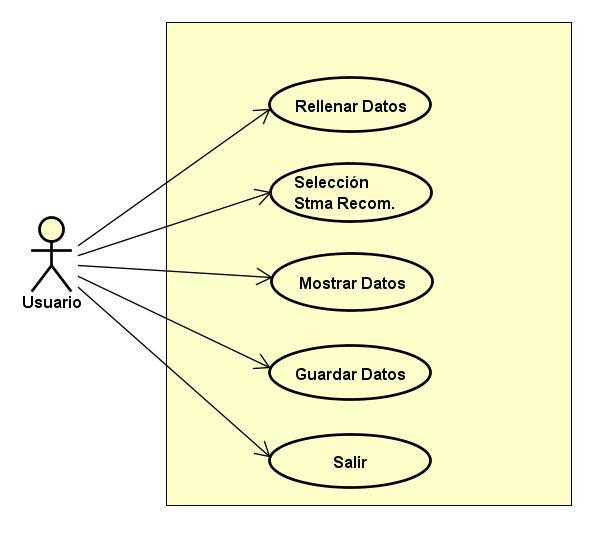
\includegraphics[width=0.90\textwidth]{Diagrama_Caso_Uso_General}
\caption{Diagrama de caso de uso General}
\label{fig:Diagrama_Caso_Uso_General}
\end{figure}